\documentclass[tikz]{standalone}
\usepackage{tikz}
\usetikzlibrary{shapes,arrows}
\usetikzlibrary{calc,positioning}
\usetikzlibrary{topaths}

\begin{document}

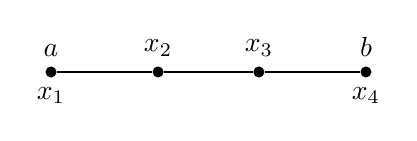
\begin{tikzpicture}
    \tikzstyle{subj} = [circle, minimum width=4pt, fill, inner sep=0pt]

    % Before diagram .........................
	\node[subj,label=below:$x_1$, label=above:$a$] (x1) at (-2,0) {};
	\node[subj,label=above:$x_2$] (x2) at (-0.64,0) {};
	\node[subj,label=above:$x_3$] (x3) at (0.64,0) {};
	\node[subj,label=below:$x_4$, label=above:$b$] (x4) at (2,0) {};	

%    \node[obj,  label=below:x] (xa) at (0,0) {};
%    \node[subj, label=below:z] (za) at (1,0) {};
%    \node[dc,   label=below:y] (ya) at (2,0) {};
	 \draw[-] (x1) -- (x2);
 	 \draw[-] (x2) -- (x3);
 	 \draw[-] (x3) -- (x4);

%    \path[-]   (za)    edge                node[swap]  {$t$}       (xa)
%                        edge                node        {$\alpha$}  (ya);

%    \node at (3,0) {$\vdash^{*}$};
%
%    % After diagram .........................
%    \node[obj,  label=below:x] (xb) at (4,0) {};
%    \node[subj, label=below:z] (zb) at (5,0) {};
%    \node[dc,   label=below:y] (yb) at (6,0) {};
%
%    \path[->]   (zb)    edge                node[swap]  {$t$}       (xb)
%                        edge                node        {$\alpha$}  (yb)
%                (xb)    edge[bend left=60]  node        {$\alpha$}  (yb);

\end{tikzpicture}

\end{document}